
\documentclass[journal]{RapportFR}

\usepackage{textcomp}

\usepackage{CJK}
\usepackage[overlap,CJK]{ruby}    % Furigana support
\renewcommand{\rubysize}{0.5}     % Furigana size
\renewcommand{\rubysep}{-0.3ex}   % Spacing between Furigana and Kanji



\usepackage[dvips]{graphicx}
\graphicspath{{./Photos/}}
\DeclareGraphicsExtensions{.eps}



% correct bad hyphenation here
\hyphenation{op-tical net-works semi-conduc-tor}


\begin{document}
\begin{CJK*}{UTF8}{min}

\title{Rapport Culturel - Japon 2011}


\author{L\'{e}o Baudouin.}

% The paper headers
\markboth{IFMA}{Shell \MakeLowercase{\textit{et al.}}: Rapport culturel sur mon stage au Japon.}

\maketitle


\begin{abstract}
%\boldmath
Ce rapport est un compte rendu des observations sur les japonais concernant leur mode de vie et leurs comportements, ainsi qu'une analyse critique des diff\'erences entre les Fran\c cais et les Japonais.

\end{abstract}

\begin{IEEEkeywords}
Stage \'etranger, Japon, AIST, rapport culturel.
\end{IEEEkeywords}



\section{Introduction}


\IEEEPARstart{U}{n} des buts des stages \`a l'\'etranger propos\'es par l'IFMA dans le cadre d'une ann\'ee de c\'esure est de d\'ecouvrir, de visiter, de comprendre et d'apprendre respectivement un pays, ses habitants et sa langue.
L'objectif culturel de ce stage \'etait de s'impr\'egner de la culture Japonaise. Confirmer ou non les id\'ees re\c cues que l'on a sur les habitants du pays du soleil levant.

J'ai effectu\'e mon stage \`a Tsukuba (つくば市), dans la pr\'efecture d'Ibaraki, au nord-est de Tokyo, dans le laboratoire Japonais AIST -- Advanced Industrial Science and Technology. La section dans laquelle j'ai travaillé, le JRL -- Joint Robotic Laboratory, \'etait compos\'e de quelques Japonais et d'une dizaine de Fran\c cais. L'anglais \'etait donc la langue officielle lors des r\'eunions ou pour les rapports. 

Ce rapport expliquera pourquoi j'ai choisi le Japon, avant d'exposer ce que j'ai retenu de la culture et du comportement des Japonais. Une partie sera consacr\'ee \`a la visite du Japon, et enfin j'expliquerai pourquoi mon s\'ejour n'a dur\'e que 30 jours.

\section{Le Japon}

\subsection{Pourquoi le Japon}

Je n'\'etais jamais sorti de France avant de m'envoler pour ce pays \`a l'autre bout de la terre. Je voulais absolument partir loin afin de conna\^\i tre un d\'epaysement total.
Le Japon a toujours \'et\'e consid\'er\'e comme un pays avec une culture unique au monde, un comportement et une vision des choses qui vont avec. Par ce voyage j'ai voulu en apprendre plus sur ce pays qui m'attirait depuis fort longtemps. 

J'ai \'egalement choisi le Japon car le sujet du stage qui m'\'etait propos\'e correspondait exactement \`a mon projet de carriri\`ere, c'est \`a dire de la recherche dans le domaine de la robotique humano\"\i de. C'\'etait l'occasion pour moi de valider mon master recherche tout en travaillant avec le CNRS, en partinariat avec le LAAS, un laboratoire français dans lequel j'envisage de faire un th\`ese. Travailler dans le pays qui est le mieux plac\'e dans ce domaine pr\'ecis ne pouvait \^etre qu'un avantage pour moi.

\subsection{Id\'ees sur le Japon avant le d\'epart}

Avant de partir, j'avais, comme tout le monde, une id\'ee pr\'econ\c cue du Japon : un pays riche en avance sur son temps, un paradis de la thechnologie. J'avais \'egalement entendu que les Japonais faisaient souvent passer leur vie professionnelle avant la vie de famille. 

En allant au Japon je souhaitais d\'ecouvrir un monde nouveau, aussi bien au niveau de l'architecture, des paysages, du mode de vie et de la langue. Je voulais me plonger dans ce pays de la robotique et des technologies. Au final seul la langue m'a vraiment d\'epays\'e, le reste \'etant assez semblable \'a la France.

\subsection{Une langue compl\`exe}

Pour pr\'eparer ce stage, j'avais pris des cours de Japonais pendant plus d'un an. Ceux ci se sont av\'er\'es quasiment inutiles une fois en face d'un vrai Japonais, étant incapable de comprendre la r\'eponse \`a la question que je venais de bafouiller. Bien que le Japonais soit une langue assez simple \`a parler (construction logique des phrases, simplicit\'e de la grammaire et de la conjugaison), les Japonais ont tendance \`a parler vite, au m\^eme titre que les Espagnols et peu se soucis d'\^etre compris par les \'etranger.

Il existe quatre fa\c cons d'\'ecrire le Japonais, deux syllabaires de base, les \textit{Hiragana} et les \textit{Katakana} (pour les mots d'origines \'etrang\`ere) comportant 46 syllabes chacun. Apr\`es un an d'apprentissage du Japonais, je comprenais ceux-ci sans difficult\'e. Cependant un troisi\`eme moyen d'écrire le Japonais existe, les \textit{Kanjis}, se sont des id\'eogrammes, qui repr\'esentent un mot ou une id\'ee. Il en existe 1975 officiels et plus de 3000 dans le language courant, autant dire que les 20 ou 30 \`a ma connaissance n'ont \'et\'e d'aucune utilit\'e. Une phrase typique Japonais m\'elange les \textit{Hiragana}, \textit{Katakana} et les \textit{Kanji}, donc il \'etait toujours impossible de lire un phrase enti\`erement. Le dernier moyen d'\'ecrire le Japonais est le \textit{Romaji}, l'\'ecriture romaine des mots Japonais, cependant celle-ci n'est utilis\'ee que pour les marques et les cours de Japonais.
Il a donc \'et\'e tr\`es dur de s'y retrouver, aussi bien dans les restaurants que dans les magasins, car tr\`es peu d'articles sont doubl\'es en anglais.

J'ai donc \'et\'e contraint de communiquer en anglais, et c'est \`a ce moment que j'ai pu me rendre compte que la plupart des Japonais ne le parlent pas ou tr\`es peu. J'ai essay\'e de poser mes questions aux \'etudiants pensant qu'ils auraient le m\^eme niveau que moi, mais sur le groupe de 5, seul un des Japonais parlait anglais. Les caissiers et caissi\`eres dans les magasins ne parlaient qu'en Japonais, il \'etait donc souvent tr\`es difficile de se comprendre.
C'est seulement au laboratoire que j'ai pu rencontrer des Japonais parlant un anglais parfait, contrastant avec ceux que j'avais crois\'e en ville.
Ceci m'a tr\`es \'etonn\'e, je pensais que la France \'etait en retard sur l'apprentissage de cette langue mais le Japon semble l'enseigner encore moins.

\subsection{Culture}


\subsubsection{Musique}

Traditionnelle,
%\begin{figure}[!t]
%\centering
%\includegraphics[width=2.5in]{Musique}
%\caption{Concert de musique dans les rues de Tsukuba.}
%\label{fig_music}
%\end{figure}
Rock,
(Pop).

\subsubsection{Coutumes}

Les r\'ev\'erences remplacent les poign\'ees de mains, il faut s'y habituer car les Japonais \'evitent au maximum les contacts. Ils vont donc faire de nombreuses r\'ev\'erences quand ils sont pr\'esent\'e \`a quelqu'un, \`a la limite de l'\'exag\'eration. Dans le m\^eme style on retour l'omnipr\'esence du ありがとうございます -- $Arigat\bar{o}~ gozaimasu$ -- merci beaucoup. Quand on rentre ou sort d'un magasin, d'un restaurant, dans le m\'etro, le bus, on ne remarque plus que \c{c}a au bout de quelques heures.

\subsection{Transports}

\subsubsection{Transport en commun}

Les services de plus sont aussi pr\'esent qu'en France, la grande diff\'erence c'est que l'on paye en descendant et non pas en montant. Il n'existe pas la fraude que l'on retouve tout le temps en France, le respect domminant tout.
Le service des trains est le m\^eme qu'en France \`a l'exception qu'il n'y a jamais de retard due \`a la ponctualit\'e exemplaire des Japonais.
Le m\'etro \'a \'et\'e plus difficile \`a utiliser, car les noms des stations n'\'etaient \'ecrit que en Japonais, avec des Kanjis. Nous avons essay\'e de trouver la station \textit{Ochanomizu} (御茶ノ水), mais il a fallu demander de l'aide afin de d\'ecripter le tableau des destinations.
L'originalit\'e du service de m\'etro est que l'on paye un montant correspondant au traject pr\'evu et que l'on ajuste \`a la sortie aux bornes "\textit{fare adjestment}" si on a \'et\'e plus loin que pr\'evu.
Tous les services de transport en commun sont propres et il y r\`egne un climat de s\'ecurit\'e contrairement \`a se que l'on peur ressentir \`a Paris.

\subsubsection{Le v\'elo}

Mode de d\'eplacement par excellence, les Japonais utilisent \'enormement ce moyen de locomotion. Nous avons pu acheter des v\'elos \`a 2000\textyen, soit l'\'equivalent d'une vingtaine d'euros. De nombreuses pistes cyclables et parking \`a v\'elos sont amm\'enag\'es en ville qui rend sont utilisation particuli\`erement agr\'eable. Il a cependant fallu un peu de temps pour se faire \`a la conduite \'a gauche qui boulversait nos habitudes et qui pouvait s'av\'erer dangereux par moment.

Dans un pays ou on ne parle pas d'\'ecologie, j'\'etais content qu'autant de monde utilisent des v\'elos se qui rendait l'air tr\`es respirable en ville, contrairement aux grandes villes fran\c caises.


\subsection{Commerces}

\subsubsection{Magasins}

A l'oppos\'e de la France, le Japon poss\`ede tr\'es peu de grandes surfaces mais une multitude petites boutiques. On y retrouve les \textit{7Eleven}, qui sont de minuscules \'epiceries ouvertes 24h/24 et 7j/7 assez pratiques pour les besoins du quotidien.
Cependant quand il s'agit de trouver des appareils \'electrom\'enag\'e cel\`a devient plus compliqu\'e. Il faut se rendre dans les grandes villes, ou alors s'adresser \`a un magasin sp\'ecialiser qui sont comme en France hors de prix.

\subsubsection{Restaurants}

Tous les restaurants proposent en vitrine une reproduction tr\`es r\'ealiste en plastique des plats qu'ils servent. C'est vraiment une bonne id\'ee comme \c ca on peut savoir ce que l'on va manger m\^eme si on ne comprend pas un seul mot du menu.
Un exemple de devanture sur la photo \ref{fig_plats}.

%\begin{figure}[!t]
%\centering
%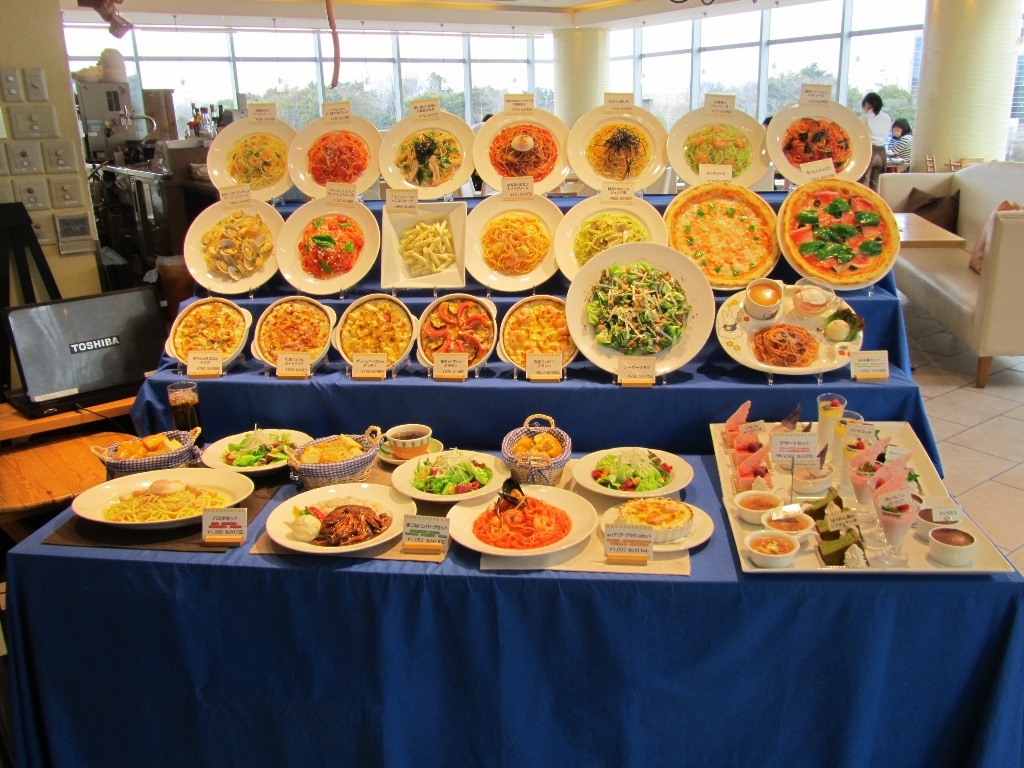
\includegraphics[width=2.5in]{Plats}
%\caption{Vitrine d'un restaurant \`a Tsukuba.}
%\label{fig_plats}
%\end{figure}

\subsection{Co\^ut de la vie}

On parle souvent du co\^ut \'elev\'e de la vie au Japon, et ce n'est pas qu'une l\'egende. Pour un europ\'een toute la nourriture est cher, que ce soit les pommes de terre \`a 70\textyen~l'unit\'e (0,70\texteuro) ou la tomate \`a 140\textyen, la viande \'egalement, il n'y a que le soja qui soit \`a un prix plus que raisonnable. Au niveau de l'\'electronique on retrouve sensiblement les m\^emes prix qu'en France dans les grandes surfaces de Tokyo. Mais il faut bien se rendre compte que si tout est plus cher, c'est qu'ils sont \'egalement mieux payer, donc pour eux les prix sont tout \`a fait normaux, mais pour les \'etrangers non pay\'es il est souvent compliqu\'e de joindre les deux bouts.

Le loyer est exorbitant, pas moyen de trouver une chambre de 9m carr\'es \`a moins de 500\texteuro/mois en ville, heureusement certaines entreprises poss\`essent leurs propres r\`esidences pour les invit\'es \'etrangers ce qui r\'eduit consid\'erablement les frais.

Les Japonais utilisent assez peu de ch\`eques ou de carte banquaire et pr\'ef\`erent tout payer en liquide, on se retrouve rapidement \`a avoir des dizaine de milliers de yen sur soi pour payer le loyer, le train, les courses et autre. Les distributeurs de l'a\'eroport de Narita ne proposent pas de billet en dessous de 10.000\textyen, l'\'equivalent d'une centaine d'euros.

\section{Le pays des contradictions}

\subsection{La t\'el\'evision}

La t\'el\'evision Japonaise est assez particuli\`ere dans le sens o\`u elle contraste totalement avec le reste de la culture.

\subsubsection{Le journal t\'el\'evis\'e}

Le Japon est connu pour \^etre le pays le plus en avance sur la technologie. Cependant en regardant le journal nous pouvons nous rendre compte qu'ils ne l'utilisent pas. Alors qu'en France les pr\'esentateurs poss\`edent des \'ecrans int\'eractifs, les Japonais eux, utilisent des posters grands formats sur lequels ils vont pr\'esenter les informations \`a l'aide d'une baguette.
Les batailles maritimes (entre la Chine et le Japon) vont \^etre expliqu\'ees \`a l'aide de petits bateaux pos\'es sur une carte de la mer de Chine.

L'explication la plus probable \`a cette non-utilisation de la technologie r\'eside dans le fait que les Japonais ont d'avantage confiance aux informations donn\'ees sur format papier. Les posters g\'eant sont donc un moyen d'utiliser cette confiance \`a travers d'autres supports m\'ediatiques.  

\subsubsection{Les jeux t\'el\'evis\'es}

Un autre aspect frappant de la t\'el\'evision Japonais sont les inonbrables jeux souvent (tr\`es) pu\'erils. Ceci contraste \'enorm\'ement avec l'image que donnent les Japonais dans la rue, une image d'hommes et de femmes s\'erieux(ses) et irr\'eprochables. 
Serait-ce un moyen de se lib\'erer des pressions accumul\'ees pendant la journ\'ee ? Je pense que c'est \'egalement fait pour retrouver le sourire, une fois chez soi, sorti du monde des convenances. 

\subsection{La nourriture}

Le Japon est \'egalement connu pour avoir le plus de centenaires au monde, ce qui est souvent expliqu\'e par l'\'equilibre des plats Japonais. Cependant la tradition se pert peu \`a peu en raison des \textit{fast-food} et des plats lyophilis\'es dont les Japonais sont grands consommateurs.

Il y a seulement quelques centaines d'ann\'ees, tout le Japon \'etait v\'eg\'etarien pour des raisons de croyances. Cependant \`a cause des importations, cette culture a quasiment disparue, les Japonais mangent d\'esormait \'enormement de viandes et de poissons. Ceci a un impact visible sur la population qui souffre de probl\`emes de digestion en autres car leurs corps ne sont pas habitu\'es \`a assimiler ces "nouvelles" substances.

La nourriture a \'et\'e mon gros probl\`eme tout le long du s\'ejour. V\'eg\'etarien depuis ma naissance, je n'ai pas souhait\'e changer pour me mettre \`a l'alimentation Japonaise. Un bon nombre de forums affirmaient qu'il \'etait parfaitement possible de ne pas manger de viande et de poisson au Japon, la r\'ealit\'e \'etait tout autre. Il fallait \`a chaque fois faire plusieur restaurant avant de trouver un menu avec un plat v\'eg\'etarien, les simples p\^ates \'etant pr\'epar\'ees dans un bouillon de poisson.
Dans les magasins les l\'egumes sont rares et chers, et les c\'er\'erales \'egalement. Nous avons donc essay\'e des l\'egumes de fournisseur locaux, ダイコン (da\"\i kon),  レンコン  (renkon), 牛蒡 (gobo) qui se sont av\'er\'es d\'elicieux.

%Contrairement aux plats tout pret du commerce

\subsection{Les coutumes vestimentaires}

Les Japonais sont connus pour \^etre d'un s\'erieux sans pariel. Il y a donc dans les rues de Tokyo des centaines de milliers de cadres en costume-cravate, mais parmis eux on peut appercevoir des personnes qui sortent du lot, comme des femmes en tenue traditionnelle, c'est-\`a-dire ...

\subsection{Architecture}

De nombreux tremblement de terre frappent r\'eguli\`erement le Japon et fragilisent peu \`a peu les b\^atiments. Il faut donc r\`eguli\`erement les d\'etruire pour en reconstruire des plus solides et respectant les nouvelles normes sismiques.
\`A cause de ces domilitions permanentes, il y a de moins en moins de maison traditionnelle comme sur la photo \ref{fig_maison}. Tsukuba est, par exemple, une ville qui m\'elange des HLM, des maisons cubiques en b\'eton, et de magnifique maisons avec des structure en bois. J'ai trouv\'e dommage que l'architecture Japonaise disparaisse comme \c{c}a au profit de maisons solides.

%\begin{figure}[!t]
%\centering
%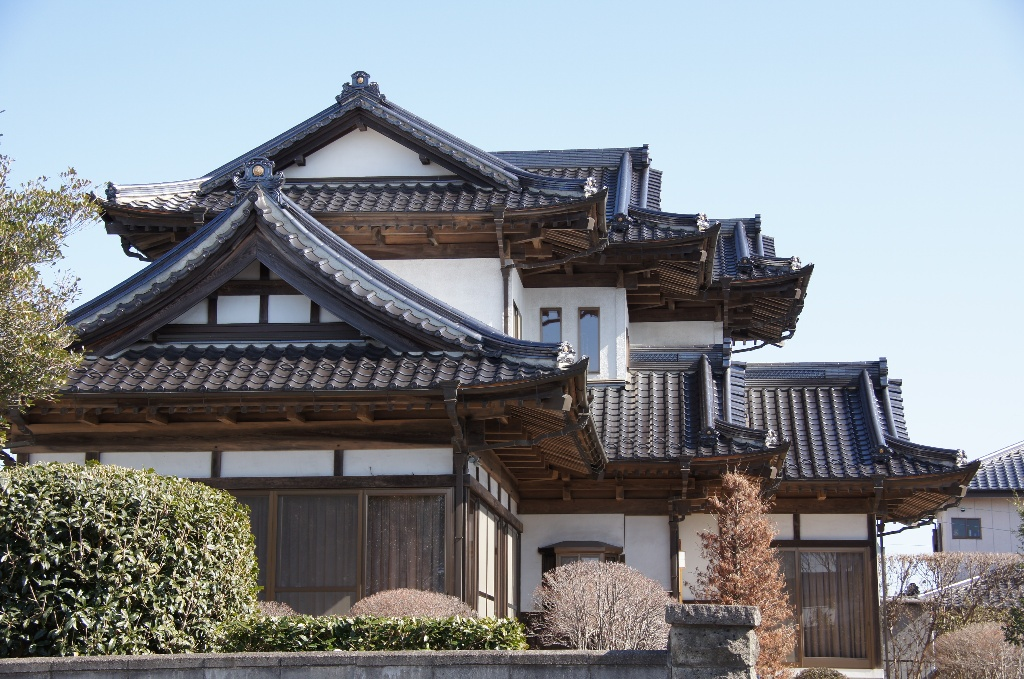
\includegraphics[width=2.5in]{Maison}
%\caption{Une maison traditionnelle \`a Tsuchiura.}
%\label{fig_maison}
%\end{figure} 

On retrouve cependant de nombreux temples cach\'es au milieu des villes comme sur la photo \ref{fig_temple} \'a 500 m\`etres des grands centres commerciaux. On y retrouve donc la totale opposition entre le nouveau Tokyo et l'ancien (Edo). 

%\begin{figure}[!t]
%\centering
%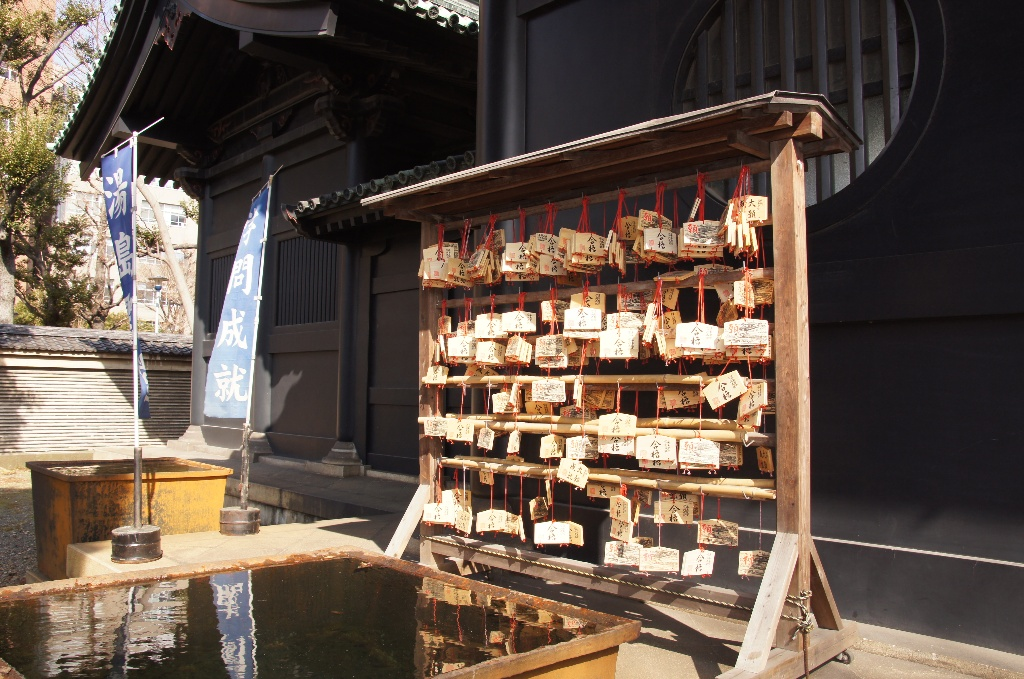
\includegraphics[width=2.5in]{Temple}
%\caption{Un temple dans le quatier d'Ochanomizu.}
%\label{fig_temple}
%\end{figure}

\section{Visite du Japon}

\subsection{Visites in\'evitables}

Le Tsukuba Express d\'essert la gare d'Akihabara, dans le quartier "\'electrique" de Tokyo (東京). On y retrouve des centaines d'immenses magasins allant jusqu'\`a 8 ou 9 \'etages, ainsi que de minuscules boutiques sp\'ecialis\'ees, (cf Photo \ref{fig_akihabara})
Arriv\'e dans les rues d'Akihabara, ce qui m'a frapp\'e c'est le calme, \`a 9h les magasins sont ferm\'es et peu de gens circulent. Cependant \`a l'heure de l'ouverture (10h), la ville s'est transform\'ee en fourmili\`ere, noire de monde.

On a retrouv\'e la m\^eme foule en soir\'ee dans le quartier de Shibuya (渋谷区), le quatier des jeunes. On y retrouve un grand nombre de magasins (v\^etement, musique, restaurant) et de \textit{Love Hotel}, h\^otels avec des chambres r\'eservables pour quelque heures seulement.

%\begin{figure}[!t]
%\centering
%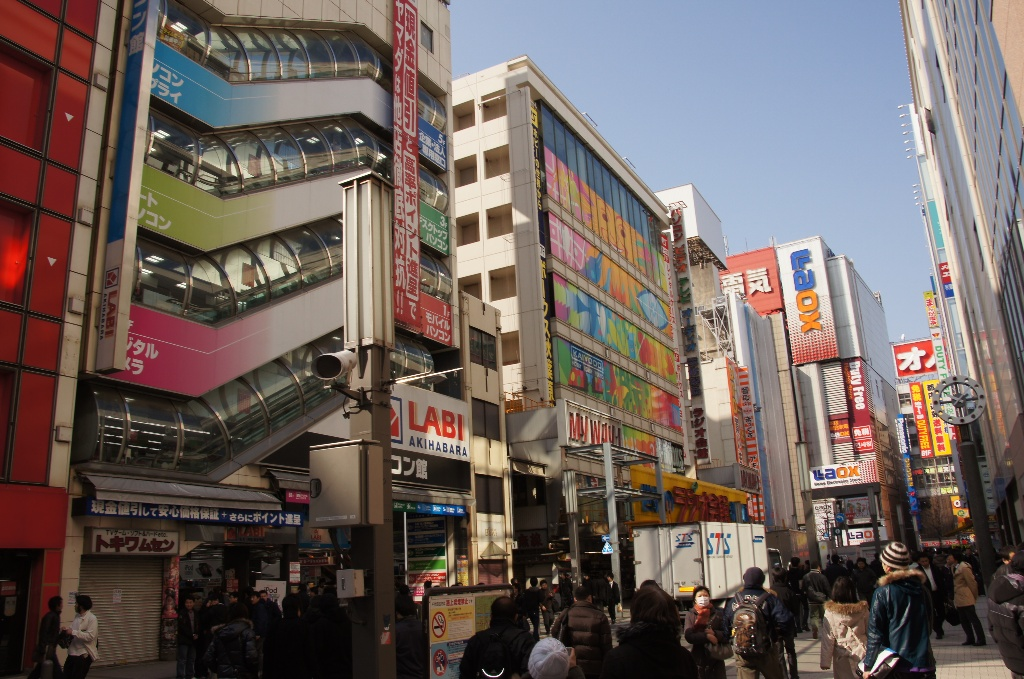
\includegraphics[width=2.5in]{Akihabara}
%\caption{Le quartier d'Akihabara \`a Tokyo.}
%\label{fig_akihabara}
%\end{figure}

\subsection{Impressions}

%\begin{figure}[!t]
%\centering
%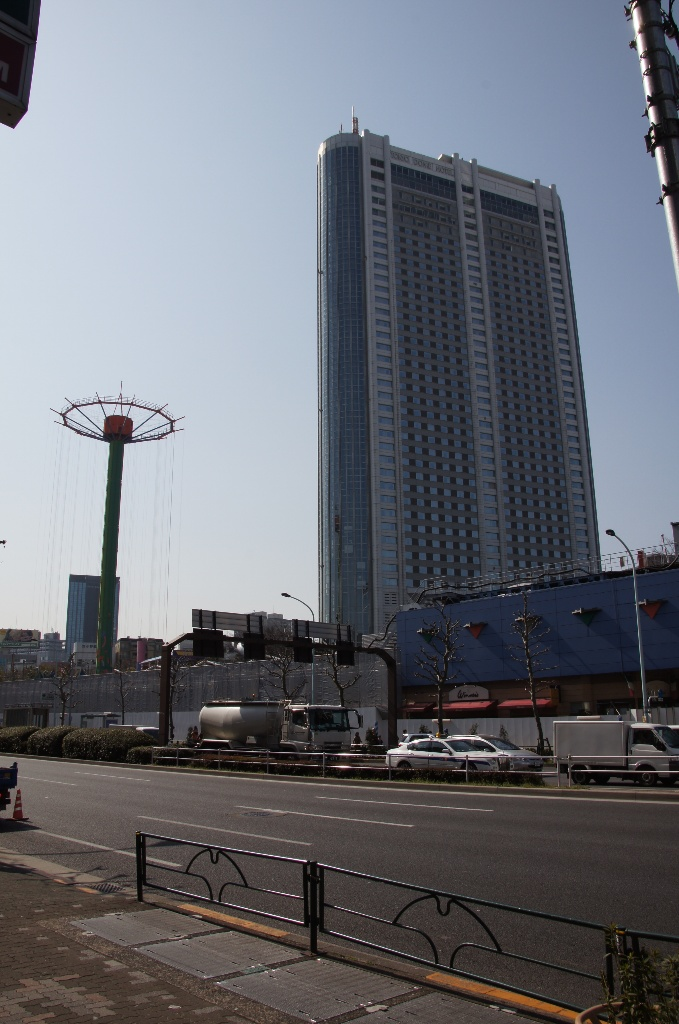
\includegraphics[height=2.5in]{GrandHotel}
%\caption{Le Grand Hotel \`a Tokyo.}
%\label{fig_hotel}
%\end{figure}

%\begin{figure}[!t]
%\centering
%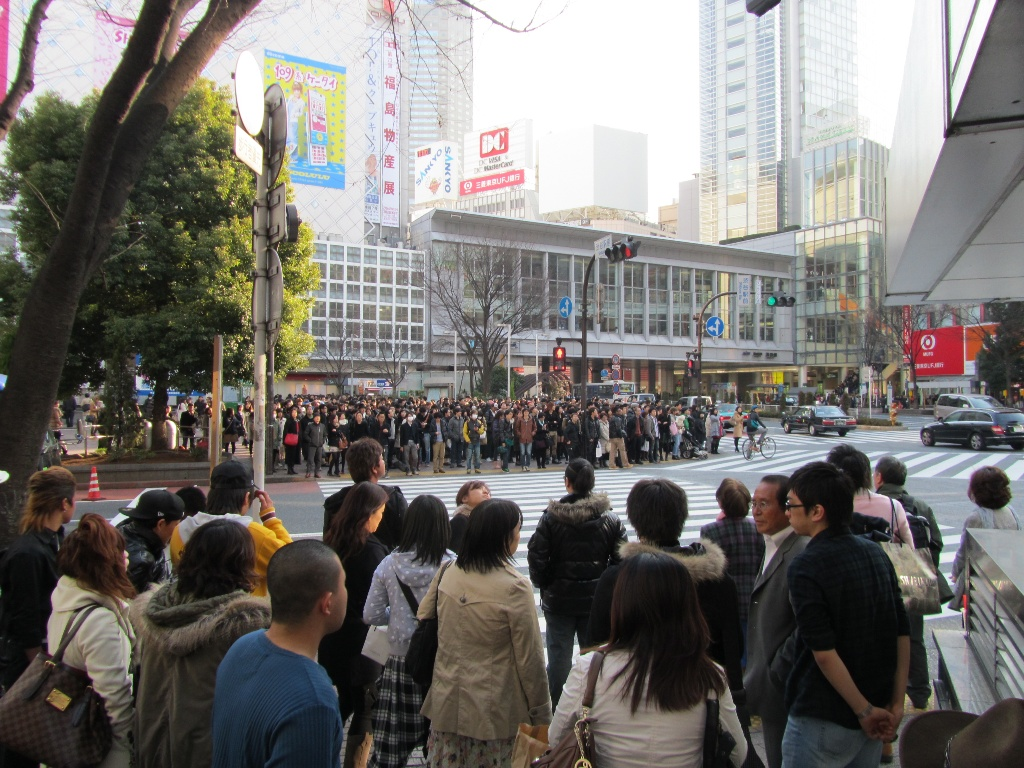
\includegraphics[width=2.5in]{Shibuya}
%\caption{Carrefour de Shibuya avant l'heure de pointe.}
%\label{fig_shibuya}
%\end{figure}

Si je devais r\'esum\'e en quelque mots Tokyo je dirai : propre, calme, immense.
Propre, car les gens ne jettent rien dans la rue, les poubelles sont en plus grand nombre qu'en France, mais aussi car les services de propret\'ee sont plus pr\'esent et vont jusqu'\`a balayer les parking pour enlever les feuilles mortes.
Calme, car les Japonais ne parlent pas dans la rue, ou alors tr\`es doucement, le parfait contraste avec les Espagnols que l'on a pu voir apr`es.
Immense, car tout est d\'emesu\'e, que se soit la taille de la ville elle m\^eme ou les batiments, comme le --Grand Hotel-- sur la photo \ref{fig_hotel}. On dirait que les building sortent de nul part. On a pu \'egalement voir le plus grand passage pi\'eton du monde \`a Shibuya pendant l'heure de pointe, il ne faut absolument pas \^etre agoraphobe. La photo \ref{fig_shibuya} a \'et\'e prise avant que l'on soit coinc\'e dans la mar\'ee humaine.

Tokyo est pourvu de magnifiques parcs qui v\'ehicule l'image des Japonais, calme et respectueux, comme celui de la photo \ref{fig_parc}.

%\begin{figure}[!t]
%\centering
%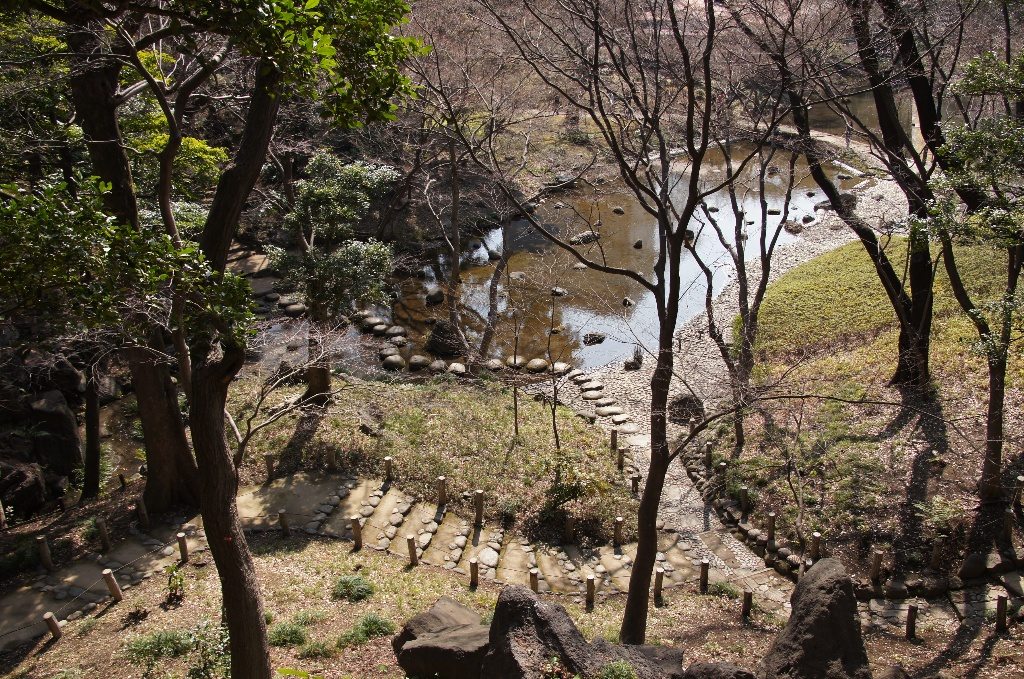
\includegraphics[width=2.5in]{Parc}
%\caption{Le parc Korakuen \`a Tokyo.}
%\label{fig_parc}
%\end{figure}

\subsection{Visites pr\'evues}

%\begin{figure}[!t]
%\centering
%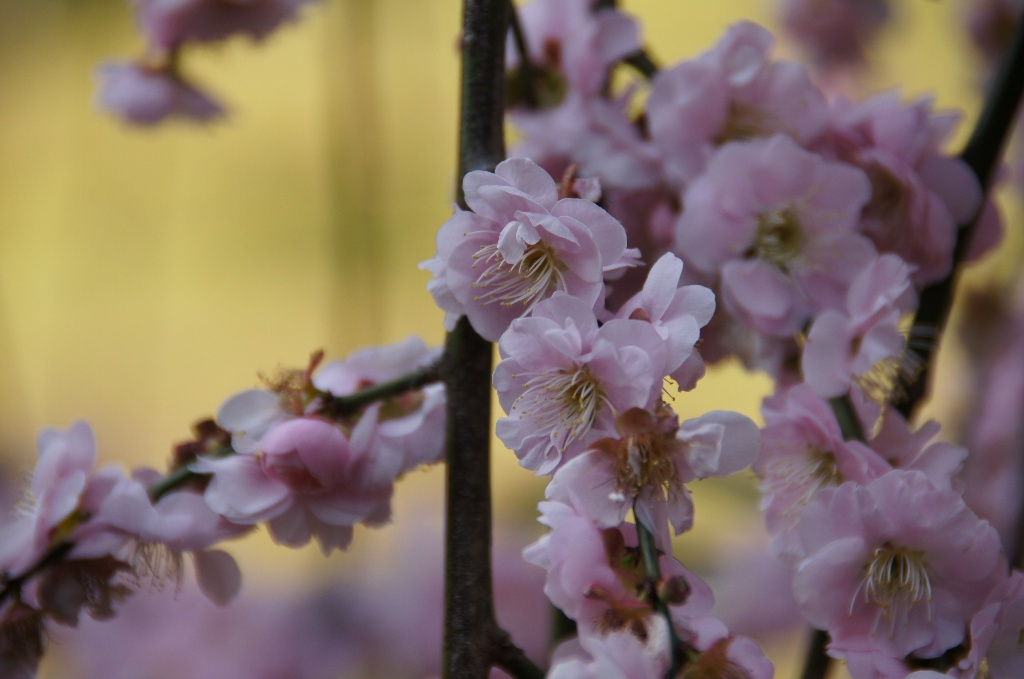
\includegraphics[width=2.5in]{Sakura}
%\caption{D\'ebut de la floraison des cerisiers \`a Tokyo.}
%\label{fig_sakura}
%\end{figure}

Suite aux incidents que j'aborderai dans le paragraphe suivant, j'ai du \'ecourter mon voyage me privant ainsi de toutes les visites que j'avais prévu.
En seulement 3 week-end, je n'ai pas eu le temps de visiter grand chose. 
La floraison des cerisier d\'ebutait juste au moment du d\'epart, je n'ai pas pu assister aux grandes f\^etes nocturnes organis\'ees sous les nuages de p\'etales rose (Photo \ref{fig_sakura}).  

J'avais pos\'e mes vacances pour la semaine suivant le tremblement de terre. Je devais aller visiter tout le sud du Japon \`a l'aide d'un billet de train sp\'ecial : 5 jours en illimit\'e.
Ce voyage pr\'evoyait des escales \`a Nagoya, Kyoto, Nara, et dans d'autres villes moins connues du sud. Je comptais y d\'ecouvrir la culture rurale Japonaise, afin de pouvoir comparer avec ce que je voyais tout les jours en ville. Je voulais \'egalement d\'ecouvrir les \textit{Onsen}, les bains d'eau chaude typiquement Japonais, et dormir dans un \textit{Ryokan}, un hot\^el traditionnel. Je devrai donc y retourner une fois dipl\^om\'e afin de connaitre les autres aspects du Japon.

\section{Incidents : s\'eisme et centrale nucl\'eaire}

\subsection{Description de l'\'ev\`enement}

Le 11 mars 2011, \`a 13h45 heure locale, un s\'eisme de forte magnitude a frapp\'e le Japon. Il s'est fait ressentir \`a des centaines de kilom\`etres \`a la ronde, comme \`a Tsukuba, \`a 300km de l'\'epicentre. Je travaillais dans le plus grand building du complexe, 8 \'etages ce qui a provoqu\'e de grandes oscillations du batiment. Au troisi\`eme, les armoires bougeaient de plus de 15cm sur place en faisant un bruit inqui\'etant. Les consignes ont vite \'et\'e donn\'ees pour se r\'efugier sous les bureaux en attendant l'accalmie, plus personne n'osait parler.
En sortant quelques minutes apr\`es nous avons pu voir que les armoire avaient \'et\'e renvers\'ees et que les peintures des murs et des plinthes avaient saut\'ees, donc que des d\'egats mineurs. C'est seulement 3 semaines plus tard que l'on a su que les cloisons du 8{\`eme} s'\'etaient effondr\'ees et qu'il y avait des fissures dans le b\'eton sous les moquettes, de quoi nous couper l'envie d'y retourner.

Pendant plus de 24h il n'y a pas eu d'\'electricit\'e \`a Tsukuba, donc il \'etait impossible de conna\^\i tre l'exitence du tsunami ainsi que l'\'etendu des d\'egats.

Une fois l'\'electricit\'e revenue nous avons pu regarder les informations \`a la t\'el\'evision japonaise, qui nous parlait d'une centrale nucl\'eaire et montrait des images d'explosions. Mon niveau en japonais ne nous permettait pas de comprendre ce qu'il se passait dans la centrale de Fukushima, \`a 200km de chez nous. Quand nous avons enfin eu internet nous avons eu acc\`es aux informations fran\c caises, qui nous ont fait peur et qui, au bout de quelques heures, nous ont convaincu de fuir le Japon pour quelques jours.
Une fois en France, nous avons appris que tout le personnel fran\c cais du JRL avait fait comme nous.

%\begin{figure}[!t]
%\centering
%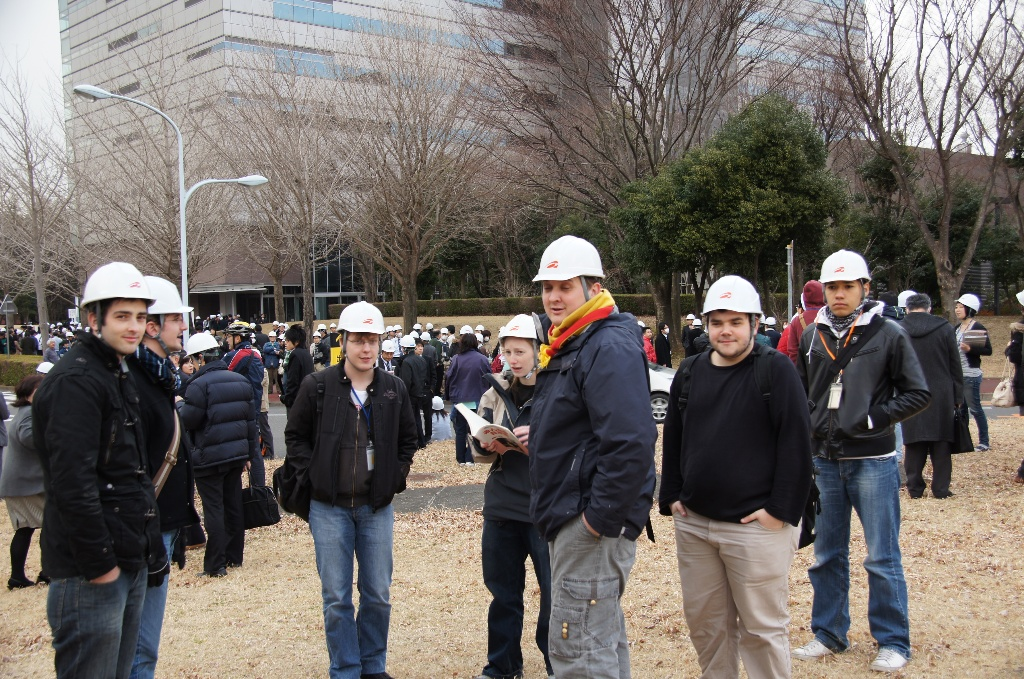
\includegraphics[width=2.5in]{Earthquake}
%\caption{Rassemblement des Fran\c cais apr\`es le tremblement de terre.}
%\label{fig_earthquake}
%\end{figure}

\subsection{Comportement des Japonais}

Les Japonais \'etaient tr\`es calmes pendant et apr\`es le tremblement de Terre, sans doute par habitude. Les Fran\c cais, eux, \'etait sur le qui-vive en redoutant toujours de fortes r\'epliques, il \'etait donc tr\`es difficile de dormir normalement. Mais je pense que l'on s'y fait assez rapidement.

Ce qui nous a le plus marqu\'e, c'est la r\'eaction des Japonais face \`a la catastrophe nucl\'eaire. Je devrais plut\^ot dire le manque de r\'eaction car ils ont une confiance aveugle dans les propos rassurants des autorit\'es, qui "maitrisaient" la situation. Seule une amie Japonaise nous a averti des risques de pluies radioactives, mais jamais d'informations officielles...

\subsection{Gouvernements Fran\c cais et Japonais}

Un des Fran\c cais a appel\'e l'ambassade afin de conna\^\i tre les consignes d'urgence. La seule r\'eponse que l'on a pu avoir c'\'etait "\textit{Achetez de l'eau et confinez vous chez vous.}". Cependant les magasins avaient d\'ej\`a \'et\'e d\'evalis\'es, et donc impossible de faire des provisions convenables.
Nous avons ensuite attendues les consignes sur internet comme conseill\'e, mais le site de l'ambassade \'etait innaccessible une fois sur deux. Nous avons appris qu'un avion avait \'et\'e mis \`a disposition pour le rapatriment des femmes enceintes et des enfants en bas \^age uniquement. Il n'y a pas eu d'autre avion gratuit pour le retour en France.
L'impression g\'en\'erale \'etait que l'ambassade nous laissait tomber et qu'il fallait se d\'ebrouiller par nous m\^eme. Nous avons donc tous eu ressenti que le gouvernement Fran\c cais ne servait \`a rien en cas de catastrophe, ce qui est relativement d\'ecevant quand on est tr\`es stress\'e comme on l'\'etait tous au Japon.

D'autre part les quelques informations donn\'ees sur le bout des doigts par le gouvernement Japonais ou l'ambassade de France, \'etaient en contradiction avec tout ce que disaient les m\'edia et les experts \'etrangers. Entre les explosions "\textit{contr\^ol\'ees}", et les r\'eacteurs qui n'ont subi aucun dommages, les mensonges \'etaient si importants que c'est ce qui nous a fait le plus peur.

La pr\'efecture d'Ibaraki est aujourd'hui la deuxi\`eme r\'egion la plus radioactive au Japon, on est donc rassur\'e d'\^etre en France aujourd'hui. Et on ne peut que plaindre tous les Japonais qui n'ont pas pu quitter leur pays.


\section{Conclusion}

N'\'etant rest\'e que 30 jours au Japon, je n'ai pas eu le temps de d\'ecouvrir ou de rencontrer assez de personnes pour que ce rapport puisse contenir tous les \'el\'ements culturels attendus.
J'ai \'et\'e tr\`es surpris et dans un sens un peu d\'e\c cu par le Japon et les Japonais en g\'en\'eral...
%Leurs fa\c con d'agir "comme des moutons" ...

%\begin{figure}[!t]
%\centering
%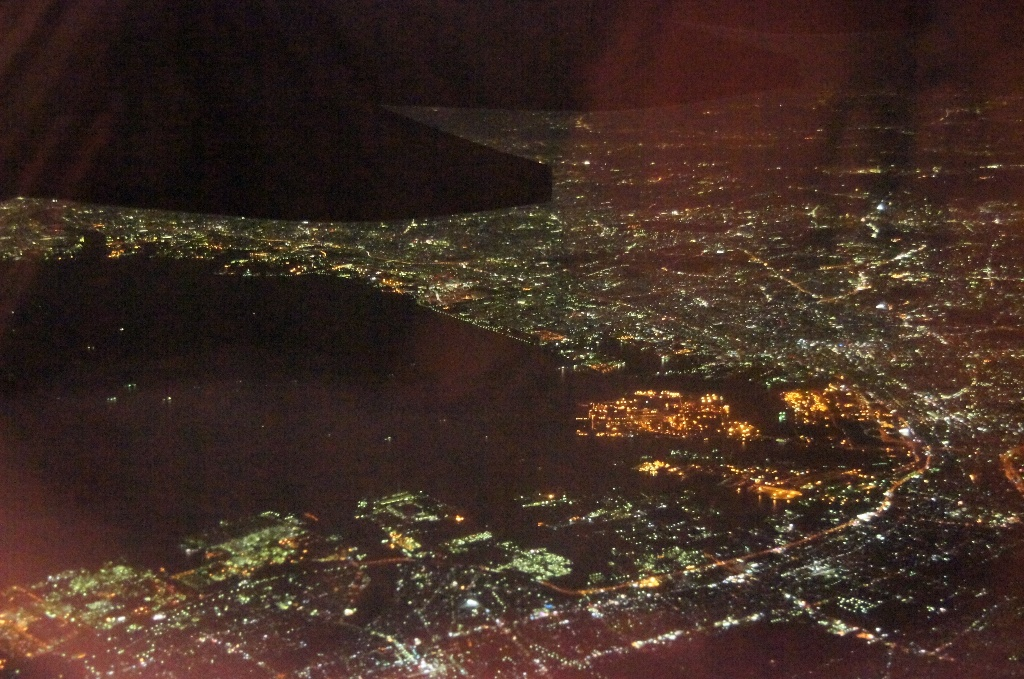
\includegraphics[width=2.5in]{Depart}
%\caption{D\'epart de Tokyo suite aux catastrophes.}
%\label{fig_depart}
%\end{figure}

La photo \ref{fig_depart} est la derni\`ere image que j'ai du Japon, avec le survol de Tokyo une ville immense, aux milliards de lumi\`eres.


\section*{Remerciements}


Merci \`a Philippe Martinet de m'avoir mis en contact avec Olivier Stasse et Eiichi Yoshida. 

Merci \`a ma compagne de m'avoir suivi dans l'inconnu \`a l'autre bout du monde sans savoir ce qu'elle allait faire une fois sur place.

Un grand merci à Nicolas Perrin, Olivier Stasse, Eiichi Yoshida, Thomas Moulard\footnote{Ce document a \'et\'e enti\`erement \'edit\'e sous \LaTeX, avec l'aide de Thomas Moulard pour incorporer les caract\`eres en Japonais.}, Sovan Nara et toutes les personnes que j'ai pu rencontrer pendant ce voyage.

\section*{Id\'ees}

\subsection{Ajouter}
%Exp\'eriences ant\'erieures,
%Contexte professionnel,
%Pr\'ejug\'es, 
%attentes, 
%nourriture, 
%musique, 
%culture, 
ambiance au travail, 
%transport en commun, 
%v\'elo, 
Tsukuba, 
AIST, 
%conduite auto, 
%payement, 
%commerce, 
ecologie, 
politique, 
%coutume (r\'ev\'erences, \textit{arigato gozaimasu}), 
%cin\'ema.

\subsection{Enlever}
%Abu Dhabi





\end{CJK*}
\end{document}


